\chapter{Case Studies}
\label{studies}

To evaluate the success of \Meta\ at supporting the addition of new language constructs, I implemented two of them, using the grammar language to extend the \Meta\ core language. The first is a simple extension of the syntax for constructing lists (one of the basic data types of the core language), and the second introduces a completely new kind of value.

%
% Definition of 'for':
%
\section{Defining the Core Language via Syntax Extension}
\label{for}
The core language is built via syntax extension on top of the kernel language, so its definitions can serve as a test of the suitability of \Meta's \keyword{grammar} facilities for building these kinds of extensions. This section compares one of the declarations from \Meta's core language with the corresponding elements from Lisp and free-form languages in terms the effort invested and the benefit accrued.

Several core language nodes provide support for using the primitive cons-list values of the Clojure platform, which are one of the basic tools for organizing data in any Lisp. These extensions employ a handful of Clojure primitives to expose the native list values of the platform, and the rest of the syntax is built around them.

%These definitions are typical of the kind of syntax extension which is used to build the elements of a language. In a Lisp, as in \Meta, this kind of syntax is reduced to the more primitive syntax of the kernel language (the special forms), whereas in a language with free-form syntax, these elements are typically built into the language's compiler. This section presents the declarations of a simple list comprehension syntax, and briefly compares the result with what would be necessary in the other approaches.

\subsection{List Comprehension in Lorax}

\begin{figure}[th]
	\centering
	
	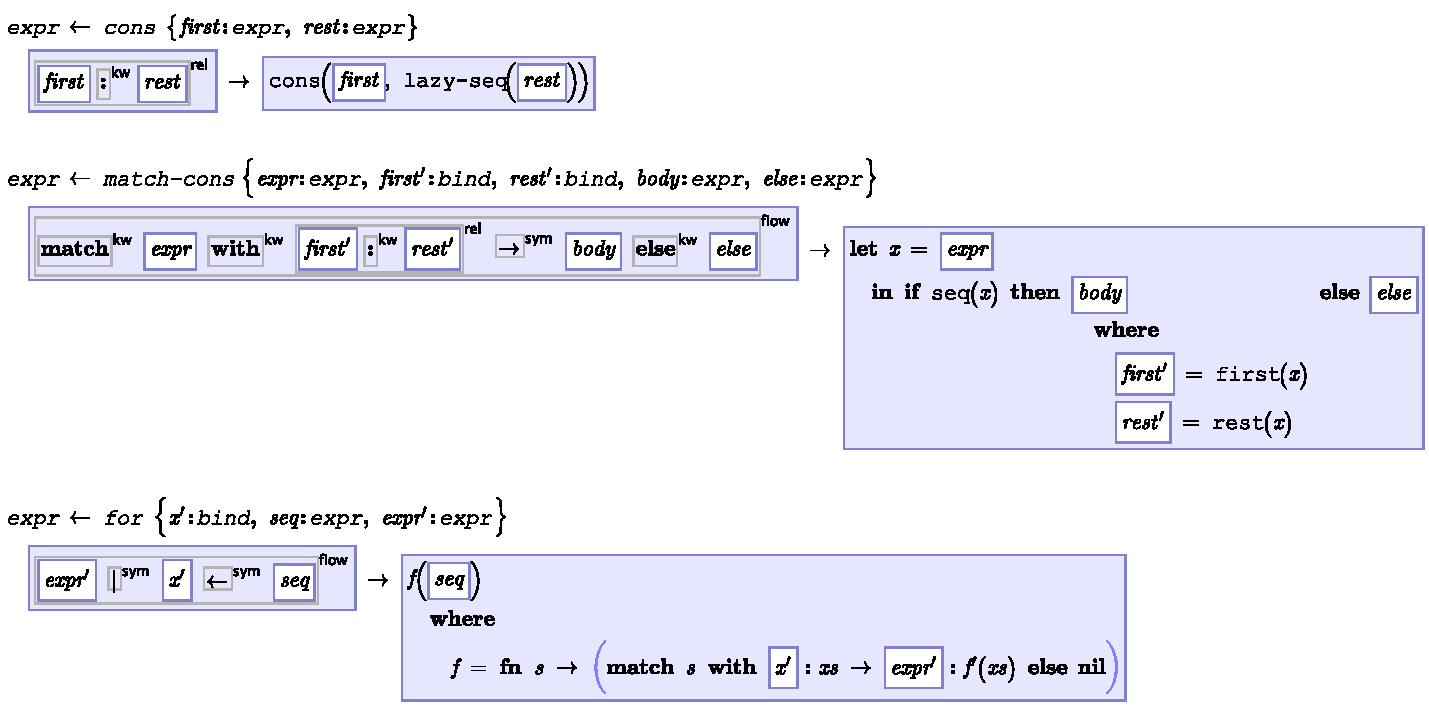
\includegraphics[scale=0.6]{src/image/cons.pdf}
	
	\caption{Declaration of the \keyword{cons}, \keyword{match-cons}, and \keyword{for} node of the core language.}
	\label{fig-for-grammar}
\end{figure}

Figure \ref{fig-for-grammar} shows the declarations of the two primitive constructs for working with with lists (\keyword{cons} and \keyword{match-cons}), and a list comprehension (\keyword{for}) node constructed from them. For the present purpose, the first two nodes can be regarded as part of the base language, and the list comprehension syntax as an extension to be added to that language.

%First is the constructor for lists: \keyword{cons}. This node, displayed as a colon operator (as in Haskell), evaluates its \keyword{first} child and uses Clojure's \clojure{cons} function to construct a cons-cell with the resulting value as its head. \clojure{lazy-seq} is applied to the \keyword{rest} child, so that it is not evaluated until the value is needed. This introduces laziness into the core language (recall that the kernel language's semantics is entirely strict), allowing infinite lists to be constructed. Note: the application of \clojure{lazy-seq} is translated by the meta-compiler to an application of the corresponding macro (with no special effort); if \clojure{lazy-seq} was treated as an ordinary (strict) function application, some additional nodes would be required to wrap \keyword{rest} in a lambda abstraction, say, to defer its evaluation.

%A \keyword{match-cons} node de-constructs a list (see the second declaration in Figure~\ref{fig-for-grammar}). Its children consist of an expression (\keyword{expr}) to be evaluated bindings for the head (\keyword{first}) and the remainder (\keyword{rest}) of the list, an expression (\keyword{body}) to be evaluated if the match succeeds, and an alternative expression (\keyword{else}) to be evaluated if the list is empty. The \emp{expand} reduction implements this by first binding the value of \keyword{expr} to $x$ (a variable local to the reduction), then applying Clojure's \clojure{seq} function, which tests whether the value represents a non-empty list. If so, the two bindings are bound to the parts of the cell using the corresponding Clojure primitive, and the \keyword{body} expression is evaluated.

%These two nodes are all that is required to construct a variety of syntax for lists, none of which will need to use the lower-level primitives. The \keyword{for} (list comprehension) node is also defined in Figure \ref{fig-for-grammar}. 
The \emp{expand} reduction for the \keyword{for} node evaluates its \keyword{seq} child, and then applies a recursive function to it. This function attempts to match its argument as a non-empty list (using \keyword{match-cons}). If so, the \keyword{x} child is bound to the first value, and \keyword{expr} is evaluated and then the function is applied to the rest of the list. Note that one of the bindings (\keyword{x}) was supplied by the programmer, and the other ($xs$) is local to the reduction. %Both \keyword{x} and $xs$ are in scope when \keyword{expr} is evaluated, thus in the new syntax, the binding introduced by \keyword{x} is in scope in \keyword{expr}, but not in \keyword{seq}.

%The rest of the core language's syntax for working with lists is defined in a similar manner, using the \keyword{cons} and \keyword{match-cons} nodes, often in combination with a recursive function to traverse the list. Some examples of the resulting syntax are shown in Figure~\ref{fig-core}. Languages such as Haskell and Python provide such features as integral parts of their fixed grammar and compiler, but in \Meta\ equal or greater expressivity is achieved with a very small implementation effort and with complete modularity---any or all of these nodes can be removed or redefined by simply editing the grammar, without any impact on the rest of the language.

\subsection{List Comprehension in Lisp}

\begin{figure}[t]
\centering
\begin{verbatim}
=> (defmacro simple-for
     [[x xs] expr]
     `((fn f# [s#]
         (if (seq s#)
           (let [[~x & r#] s#]
             (cons ~expr
               (lazy-seq (f# r#))))))
         ~xs))

=> (simple-for [x (range 1 11)] (* x x))
(1 4 9 16 25 36 49 64 81 100)
\end{verbatim}

\caption{List comprehension macro in Clojure}
\label{fig-for-lisp}
\end{figure}

For comparison, the definition of a Clojure macro with equivalent capability is shown in Figure~\ref{fig-for-lisp}. The macro operates in a very similar way to the \Meta\ syntax declaration, so a fairly direct comparison of the two is revealing. The two declarations, and the resulting syntax, differ in several ways.

Both declarations make use of quasi-quoted syntax to construct a reduced program fragment. In \Meta, the rendering of quoted nodes using a contrasting background color provides a clear visual cue of the embedded structure. It's clear at a glance where the three components of the syntax are substituted into the reduced program. In Clojure, quotation and un-quotation are indicated with lexical signifiers (as in `\clojure{`(\dots)}' and `\clojure{\textasciitilde x}'), and it's up to the reader to count parentheses to understand what is evaluated when. To avoid unintended variable capture, names introduced in the Clojure reduction are marked with another signifier (as in `\clojure{x\#}') which causes a new name to be generated each time the quotation is evaluated. In \Meta, no such signifiers are needed, because variable references are unambiguous---the meta-compiler takes care of generating new, unique labels when the quotation is expanded.

Thus the reduction/macro is of roughly equivalent complexity in the either system, but \Meta's handling of quotations and variable references makes the reduction both easier to read (via visual cues) and easier to write (by avoiding subtle issues of variable capture).

\subsection{Concrete Syntax}
In addition to this definition of semantics, \Meta's declaration defines a new syntax for the comprehension, which is designed to be familiar from both the mathematical notation of set theory and the comparable construct in Haskell. In \Meta, the reduction for this syntax is entirely trivial, simply giving the arrangement of the three child nodes and the symbols to be placed between them. The effort involved to provide such a simple reduction is essentially nil. For the programmer using the extended language, this syntax gives list comprehensions a distinct appearance, aiding comprehension. 

Returning to Clojure, the new syntax is identical to any other element of the language, with little more than the name ``simple-for'' distinguishing it from any other expression. A more illustrative comparison is with Haskell's similar construct. In Haskell, one can write the same example as follows:
\begin{verbatim}
[ x^2 | x <- [1..10] ]
\end{verbatim}
which has the same basic structure as the \Meta\ version, except that it suffers slightly for being limited to the ASCII character set.

However, Haskell's list comprehension syntax is baked into the compiler, and the programmer has no ability to add a new syntax of this kind without modifying the Haskell compiler's front-end. This is typical of languages with free-form syntax; what the language provides may work well, but the specification of syntax is inaccessible to the user (i.e.~it's outside the reach of what can be accomplished with a reasonable effort).

\subsection{Evaluation}
\Meta's facilities for declaring new syntax and specifying semantics and concrete syntax allow new syntax to be introduced with an effort that compares well to Lisp's macro facility. However, both the declaration of the new syntax and its use are significantly more readable than the corresponding Lisp programs, or even the syntax from Haskell which is designed for just this purpose. Meanwhile, the effort involved is much less than the effort would be to add such a construct to a language such as Haskell.


%
% Runtime (enumerating the rationals):
%
\section{Introducing a New Runtime Value}
The preceding section showed how the facilities of the platform can be exposed and wrapped in a novel syntax. This syntax helps the programmer to understand the program, but as soon as the program is reduced to the kernel language for evaluation, the syntax is gone and only the primitive values remain. A more ambitious goal for syntax extension is to augment the language with a new kind of runtime value. This allows programs to operate on a new kind of data, and allows the programmer to see results of computation in the natural form. The next example shows how a new kind of value can be introduced, and how it supports writing a program in a much more natural and comprehensible way.

\subsection{Enumerating the Positive Rationals}
In a delightful Functional Pearl \cite{gibbons}, Gibbons et al.\ present a series of Haskell programs which generate the infinite series of all positive rational numbers. They begin with the idea of traversing the infinite matrix $a_{ij} = i/j$ which contains every positive ratio, but also contains many equivalent, unreduced ratios (e.g. $\nicefrac{1}{2}$, $\nicefrac{2}{4}$, $\dots$).
%$$
%%\left(
%\begin{array}{cccccc}
%\nicefrac{1}{1} & \nicefrac{2}{1} & \nicefrac{3}{1} & \cdots & \nicefrac{m}{1} & \cdots
%\\
%\nicefrac{1}{2} & \nicefrac{2}{2} & \nicefrac{3}{1} & \cdots & \nicefrac{m}{1} & \cdots
%\\
%\vdots
%\\
%\nicefrac{1}{n} & \nicefrac{2}{n} & \nicefrac{3}{n} & \cdots & \nicefrac{m}{n} & \cdots
%\\
%\vdots
%\end{array}
%%\right)
%$$
%Because every integer appears in the denominator in one column and in the numerator in one row, it's apparent that the matrix contains every positive rational. Concatenating the diagonals
%($\nicefrac{1}{1}$), 
%($\nicefrac{1}{2}$, $\nicefrac{2}{1}$), 
%($\nicefrac{1}{3}$, $\nicefrac{2}{2}$, $\nicefrac{3}{1}$), 
%$\cdots$
%gives an infinite series containing all the rationals, and is easily done in constant space. However, this method has two drawbacks in that the rationals are not in reduced form and each equivalent rational is produced many times (for instance, notice that the diagonal $\nicefrac{1}{1}$, $\nicefrac{2}{2}$, $\nicefrac{3}{3}$, $\cdots$ contains only ratios equal to 1).

The authors show that a series containing all positive rationals in reduced form, without duplicates, is obtained by iterating the function 
$x' = 1/{(\lfloor x \rfloor + 1 - \{x\})},$\footnote{In the authors' notation, $\lfloor x \rfloor$ is the floor, or whole-number part of $x$, and $\{x\}$ is the fractional part: $\{x\} = x - \lfloor x \rfloor$, $x > 0$.} beginning with $x=1$. This is a surprisingly simple expression, but it is somewhat computationally undesirable in that calculating $\lfloor x \rfloor$ and $\{x\}$ involves division.

%The series begins:
%\begin{eqnarray*}
%&&1
%\\
%(\lfloor 1 \rfloor + 1 - \{1\})^{-1} 
%= (1 + 1 - 0)^{-1} 
%&=& \nicefrac{1}{2}
%\\
%(\lfloor \nicefrac{1}{2} \rfloor + 1 - \{\nicefrac{1}{2}\})^{-1} 
%= (0 + 1 - \nicefrac{1}{2})^{-1} 
%&=& \nicefrac{2}{1}
%\\ 
%(\lfloor 2 \rfloor + 1 - \{2\})^{-1} 
%= (2 + 1 - 0)^{-1} 
%&=& \nicefrac{1}{3}
%\\ 
%(\lfloor \nicefrac{1}{3} \rfloor + 1 - \{\nicefrac{1}{3}\})^{-1} 
%= (0 + 1 - \nicefrac{1}{3})^{-1} 
%&=& \nicefrac{3}{2}
%\\ 
%(\lfloor \nicefrac{3}{2} \rfloor + 1 - \{\nicefrac{3}{2}\})^{-1} 
%= (1 + 1 - \nicefrac{1}{2})^{-1} 
%&=& \nicefrac{2}{3}
%\\ 
%(\lfloor \nicefrac{2}{3} \rfloor + 1 - \{\nicefrac{2}{3}\})^{-1} 
%= (0 + 1 - \nicefrac{2}{3})^{-1} 
%&=& \nicefrac{3}{1}
%\end{eqnarray*}
Interestingly, this formula can be implemented using only ``a constant number of arbitrary-precision integer additions and subtractions, but no divisions or multiplications'' by choosing a different representation for ratios. It happens that the five necessary operations---reciprocal, floor, addition of an integer, negate, and fractional part---can all be efficiently performed on ratios represented as \emp{regular continued fractions}. A continued fraction has the form\footnote{Incidentally, this expression is a frequently-cited exception to \TeX's rules for formatting fractions---all the nested expressions are best typeset at the same size, to emphasize the recursive structure. \Meta\ does not provide a way to override that behavior, so continued fractions do not look quite this nice in \Meta!}
$$a_0 + \frac{1}{
    \displaystyle a_1 + \frac{\displaystyle 1}{
        \displaystyle \cdots + \frac{\displaystyle 1}{
            \displaystyle a_n}}}$$
A regular continued fraction is one in which all the coefficients except $a_0$ are positive, and $a_n > 1$ (except for the special case 1). Every rational has a unique representation as a regular continued fraction.

Having arrived at this elegant result, the authors proceed to reduce their formulas to the notation of Haskell for implementation, using lists of integer coefficients to represent continued fractions. In the process, the origins of the code are completely obscured by the loss of the original notation. For example, one of four cases for negation of a regular continued fraction looks like this:\footnote{Actually, what's shown in the paper has been pretty-printed for publication \cite{lhs2tex}. In the actual source code, it must have looked something like this: \clojure{negatecf [n\_0, 2] = [-n\_0-1, 2]}.}
%$$\mathit{negatecf} (n_0 : 1 : n_2 : ns) = (-n_0 - 1) : (n_2 + 1) : ns$$
%$$-\left(n_0 + \frac{1}{\displaystyle 1 + \frac{1}{n_2 + \cdots}}\right) = (-n_0 - 1) + \frac{1}{(n_2 + 1) + \cdots}$$
$$\mathit{negatecf}\:[n_0, 2] = [-n_0-1, 2]$$
It's up to the reader (of the paper or of the code) to decode the representation of fractions being used here and work out how this corresponds to the algebra that motivated it. However, in the proper notation, the same definition reads as simple algebraic equation which is easily understood and checked:
$$-\left(n_0 + \frac{1}{2}\right) = (-n_0 - 1) + \frac{1}{2}$$
The awkwardness of Haskell's notation is an impediment to understanding the program as an artifact, but it also obscures the program's meaning in a more subtle way. The choice of integer lists as a representation, as opposed to defining a new algrebraic data type with a similar recursive structure, was probably driven by the relative economy of the notation for lists (which is provided by the Haskell parser as a special case). As a result, accurate type information is lost, which makes the program harder to understand both in the writing and at runtime.

%\vspace{12pt}

\subsection{Continued Fractions in \Meta}
In \Meta, one can extend the language with a new kind of value for these fractions. I did this by defining a \keyword{continuedFraction} node which defines a recursive data type. It is displayed in the obvious way, except that when the continuation is the ``null'' value, it is displayed in a slightly simplified form. The \emp{expand} reduction is new---it reduces to an expression which evaluates the component expressions and then constructs a node. Therefore the node itself becomes a runtime value. Several \keyword{match} nodes provide pattern matching on the runtime shape of the argument, and are used to identify the cases in each operation. Figure~\ref{fig-cf} shows the declarations of the five operations, and some simple examples of their use are shown in Figure~\ref{fig-cfex}.
\begin{figure}[th]
  \centering
  
%  \todo{split into columns?}
  
  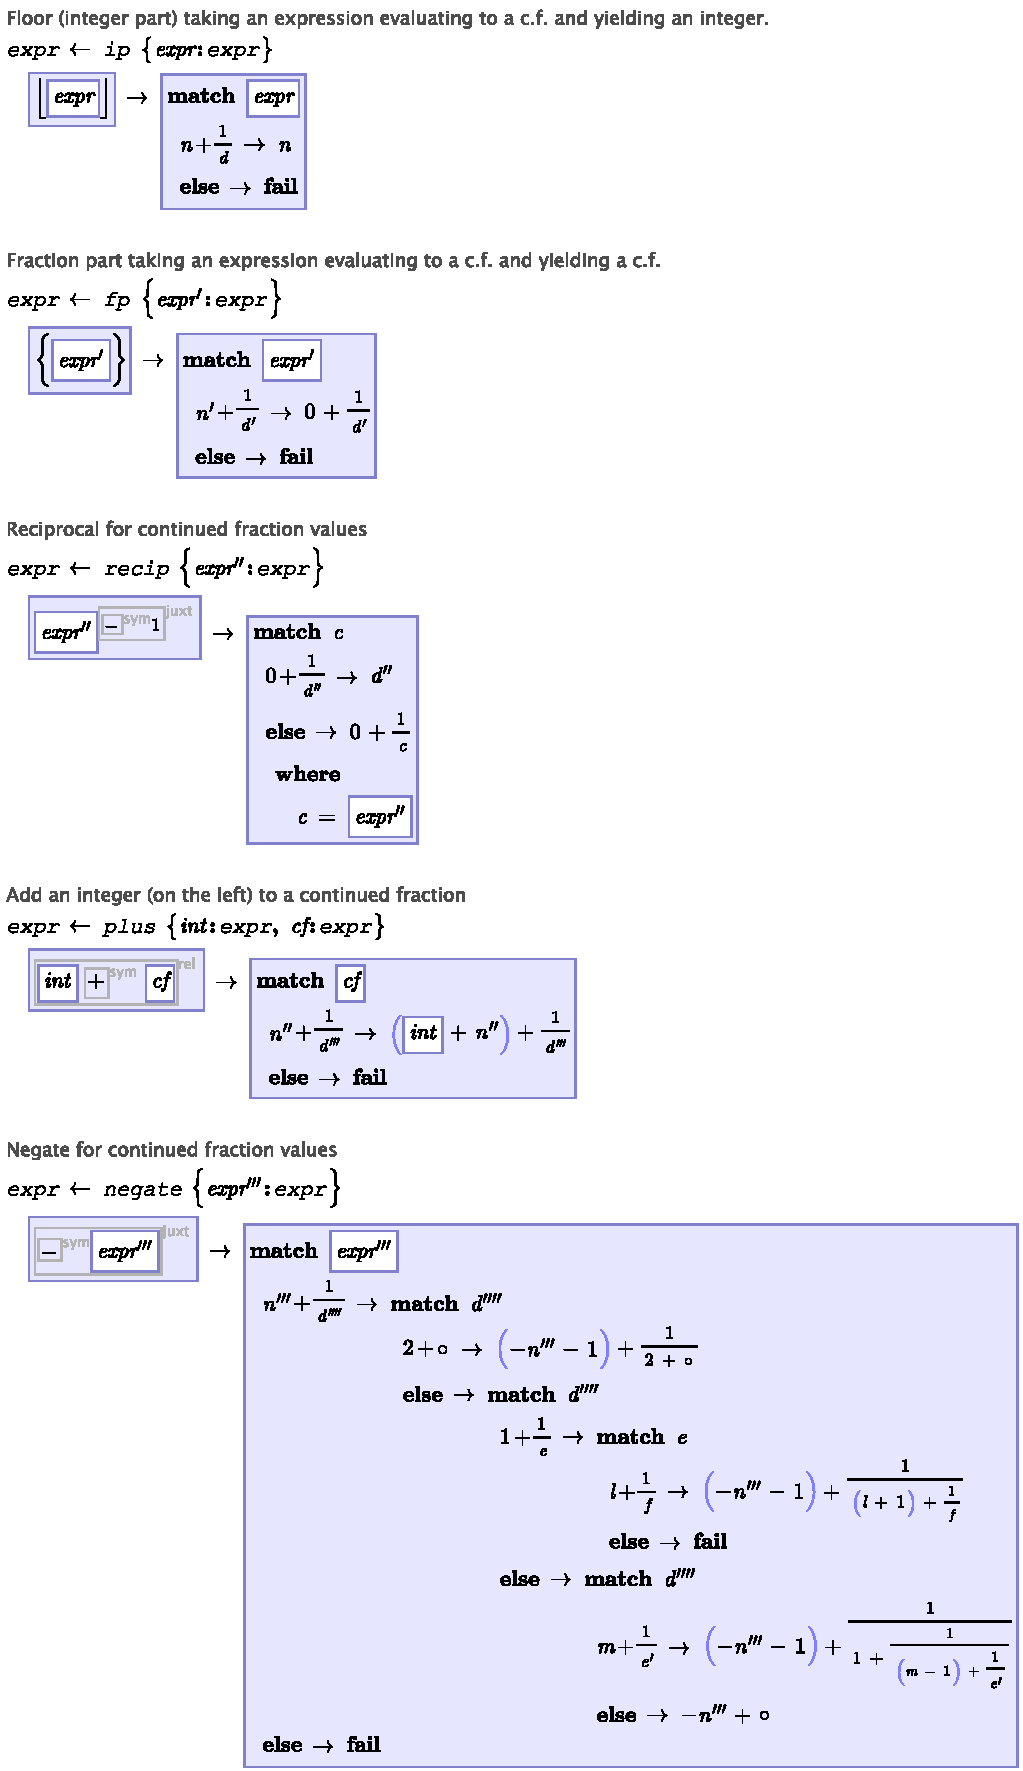
\includegraphics[scale=0.5]{src/image/continued-ops.pdf}
  
  \caption{Grammar for operations on continued fractions as runtime values.}
  \label{fig-cf}
\end{figure}

\begin{figure}[th]
  \begin{center}
  
  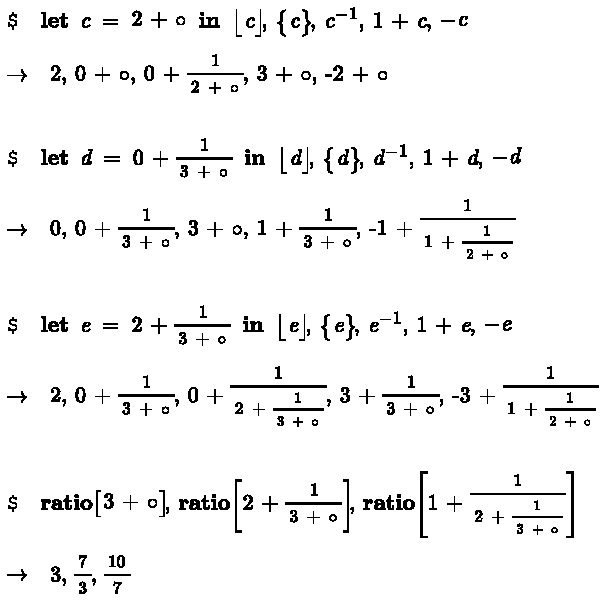
\includegraphics[scale=0.8]{src/image/continued.pdf}
    
  \end{center}
  \caption{Operations on continued fractions.}
  \label{fig-cfex}
\end{figure}

Note that these declarations are somewhat straining the current capabilities of \Meta. Ideally the construction of a runtime node would be as simple as adding a second level of quotation to the \keyword{expand} reduction, but the current prototype does not handle that properly, so a bit of extra ceremony is required. In fact, in order to achieve the relatively understandable reductions shown in Figure~\ref{fig-cf}, I had to manually define a total of seven different \emp{match} nodes, out of a possible 16 for patterns up to three levels deep. It would be much more convenient to have a general pattern-match construct supporting multiple patterns, each a node with bindings substituted for some of the child nodes, but \Meta's current approach to reductions cannot handle that. Nevertheless, with the hard work of defining syntax and semantics out of the way, the actual algorithm can be expressed quite naturally.

The expression which produces the next fraction in the series is wrapped in a function:
\begin{center}
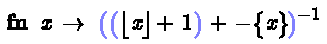
\includegraphics[scale=1]{src/image/rationals-next.pdf}
\end{center}
Note that in this form the expression does not exactly match what was shown earlier, because some algebraic manipulation is necessary to put it into a form that uses only the operations that have been defined. The resulting expression contains one node (operator) for each operation to be performed. For instance, the original expression hid a negation and an addition operation behind a single $-$ symbol, but my version makes the two operations explicit. Also, \Meta\ inserts a pair of parentheses to clarify the order of evaluation of the two addition operations, another point which is left to algebraic convention in the original. Other than that, my choice of notation resembles the original precisely.

Now generating the infinite series in continued fraction form is as simple as applying the \emp{iterate} operator (${}^*$) to the $\mathit{next}$ function, using 1 as the initial value:
\begin{center}
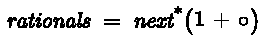
\includegraphics[scale=1]{src/image/rationals-iter.pdf}
\end{center}
The complete expression and the first 15 fractions (converted to simple ratios) appear in Figure~\ref{fig-rationals}. 

% todo: more of a punchline?

\begin{figure}[t]
  \centering
    
  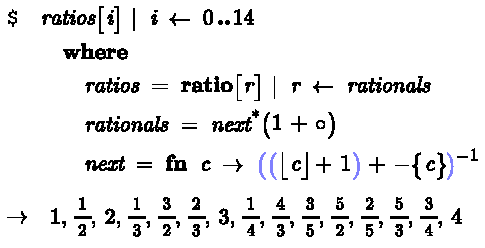
\includegraphics[scale=0.8]{src/image/rationals.pdf}
  
  \caption{Enumerating the rationals, using continued fractions.}
  \label{fig-rationals}
\end{figure}

\subsection{Evaluation}
\Meta\ allows a novel runtime value to be defined entirely in terms of nodes and reductions. Once a constructor and some syntax for pattern matching on the new values are defined, it's quite straightforward to implement operations on the new values, and to write programs which make use of the values and operations on them.

In the case of continued fractions, the notation is clearly superior to what can be done in a textual language, in terms of aesthetics and ease of understanding. Furthermore, the improved notation encourages the use of a proper data type, as opposed to the awkwardness of Haskell which pushes the programmer towards using a generic data type which is slightly more convenient.

One thing to note is the use of identical $+$ symbols for two distinct addition operations (first addition of integers, and then addition of an integer to a continued fraction). It might be preferable to use a different symbol for the new kind of addition. Because that symbol is specified in one place---the presentation reduction for that node---it's trivial to make the switch. On the other hand, this may be a case where some ambiguity in the visual representation can actually enhance readability. If that freedom leads to an incorrect program, it's easy to click on either node and the editor will indicate which $+$ is of which type. Alternatively, one might want to use the same kind of ``plus'' node for either operation and have the correct implementation determined automatically (either by analyzing the types or by checking the values to runtime). The latter approach is in fact what Clojure's built-in \clojure{+} operator does for integer, floating-point, and rational values, but \Meta\ does not currently attempt to provide such a mechanism.

However, the current limitations of \Meta's approach to reductions make the job of defining these operations more arduous than it should be. A more general mechanism for implementing pattern-matching is needed to make this attractive.

\section{Final Notes}
Online syntax checking is a significant boon to developer productivity (as evidenced by the general adoption of syntax-highlighting editors and interactive-compiling IDEs), and \Meta\ provides much of the benefit of this technique through its simple grammar language. However there is one place where this checking is not effective: the contents of quoted nodes may have any type whatsoever, and an un-quote node must be allowed to appear anywhere at all. This is a consequence of the fact that \Meta\ grammars specify only local structure. For example, to properly constrain the nodes of a presentation reduction, it would be necessary to require that the value produced by the reduction is a node in the presentation language. As it is, this kind of error is not discovered until runtime (i.e. when the editor attempts to apply the reduction). And lacking this kind of information, the editor is not able to provide reasonable suggestions when editing quote nodes. This is a significant gap, but adding what amounts to a type system to \Meta\ for this purpose alone seemed ill-advised. Of course, many of the languages people want to use are statically typed, so a more complete system will probably need to solve that problem anyway.

The most significant limitation of \Meta\ as a practical tool is its lack of integration with existing tools. The prototype editor could be developed into a stand-alone tool, and it could perhaps be used to generate traditional source or object code for use with another system. A more ambitious goal would be to integrate this style of editing into an existing IDE. Ultimately, many other integration points would need to be addressed, including most obviously source code management, but also any and all tools that aim to present or analyze source code.